%
% ======================================================================
\RequirePackage{docswitch}
% \flag is set by the user, through the makefile:
%    make note
%    make apj
% etc.
\setjournal{\flag}

\documentclass[\docopts]{\docclass}

% You could also define the document class directly
%\documentclass[]{emulateapj}

% Custom commands from LSST DESC, see texmf/styles/lsstdesc_macros.sty
\usepackage{lsstdesc_macros}

\usepackage{graphicx}
\graphicspath{{./}{./figures/}}
\bibliographystyle{apj}

% Add your own macros here:



%
% ======================================================================

\begin{document}

\title{ The LSST DESC Data Challenge 1: Generation and Analysis of Synthetic Images for Next Generation Surveys }

\maketitlepre

\begin{abstract}

The success of the Large Synoptic Survey Telescope (LSST) as a dark energy experiment will depend on controlling systematic effects for the various cosmological probes.  Simulations are critical for developing the methodology to estimate and mitigate these systematics.  In the first Data Challenge from the LSST Dark Energy Science Collaboration, we evaluate the potential systematic effects that will affect observables, with an emphasis on galaxy clustering.  We utilized two approaches to simulate LSST images, one of which (PhoSim) involves fully realistic ray-tracing.  Simulated images were then processed, combined, and analyzed using the current version of the LSST Data Management pipeline.  Here we characterize the resulting systematics and implement corrections.  Our results demonstrate that we can generate realistic LSST-like simulated images and control the systematic effects, after processing these images, at a sufficient level to enable major advances in our knowledge of dark energy and cosmology. The methodology presented here can be easily translated to current and future imaging surveys.
\end{abstract}

% Keywords are ignored in the LSST DESC Note style:
\dockeys{LSS , Data challenge, Systematics}

\maketitlepost

% ----------------------------------------------------------------------
%

\section{Introduction}
\label{sec:intro}

One of the most critical aspects in Stage IV experiments is the characterization of their instrumentation and systematic effects~\citep{2006astro.ph..9591A}. In the case of  LSST~\citep{Overview,ScienceBook,WhitePaper} this becomes especially difficult given its wide variety of cosmological probes. In this paper we present a methodology to characterize the LSST large-scale structure (LSS) transfer function and an analysis of potential systematic effects present in LSS analyses.
% ---------------------------------------------------------------------

\section{Formalism}

In this section we will present the formalism to characterize the LSST transfer function. \CHECK{Write the formalism. For full sky $C_{l,output}=T_{l}C_{l,input}$ where $T_{l}$ is the transfer function, but for partial sky measurements this is more complicated. We can also try to use $P(k)$ where the transfer function is straightforward to measure. If we use correlation functions maybe we just want to use the angular correlation function instead of the comoving distance-based correlation function}.

% ----------------------------------------------------------------------

\section{DC1 data}
\label{sec:data}
In this section we describe the dataset. For now we have two possibilities: the \texttt{ImSim} catalog which is based on the LSST GalSim package and the \texttt{PhoSim} catalog. Both of them use as an input the CatSim catalog. This catalog is based on the dark matter haloes from the Millenium simulation and a semi-analytic baryon model described in \citep{2006MNRAS.366..499D}. This catalog covers a redshift range from $0 < z < 6$ covering a $4.5 \times 4.5$ degree footprint on the sky which is the equivalent to the LSST field-of-view. It has a higher number density of galaxies than the expected for LSST, since it contains sources fainter than the detectable limits for LSST. This is very useful to study the detection limits of LSST. This simulation also contains stars represented as point sources and drawn from the Galfast model~\citep{2008ApJ...673..864J}. CatSim also contains associates each source with an SED.

In total the input catalog to both \texttt{ImSim} and \texttt{Phosim} contains $N$ sources of which, $N_{gal}$ are galaxies and $N_{star}$ are stars. Using this catalog the Survey Simulations Working group generates 4 exposures of the full LSST focal plane in the r-band. These four exposures are simulated both using GalSim~\citep{2015A&C....10..121R}, and PhoSim~\citep{2015ApJS..218...14P}. The \texttt{ImSim} (GalSim) simulation has a big speed advantage but it lacks of some important effects on the sensor such as cross-talking or pixel saturation. For comparison, the focal plane simulation takes approximately 1 week using GalSim whereas it takes slightly longer than a month using \texttt{PhoSim}. \CHECK{Add more information about the catalog and some plots}.

The outputs of these simulations are then processed using the LSST data management (DM) stack~\citep{Overview,ScienceBook,WhitePaper}  \CHECK{Is there any other reference for the stack?}. The DM stack is intended to be the software used to process the data produced by LSST. Although it is still under development, most of the pieces are already meeting the science requirements or very close to do that. Running the DM stack on this dataset also constitutes a necessary test for this invaluable piece of LSST. The stack can be divided into three main steps: the coadding step where the images are put together to form a deeper image than each individual exposure; the detection step, where the coadded image is analyzed searching for peaks on the counts; and the measurement step, where these peaks are characterized. The DM stack performs these three steps automatically and provides an image and a source catalog with $N_{sources}$ and the following columns: $X$ \COMMENT{Depending on the extensions used at the time of DC1 we will have a different number of columns, i.e., if you use the shape measurement extension you have extra columns with the GalSim shape measurement results. You can also have extra columns with the Kron photometry extension.} 

We show a small patch of the generated coadd in \figref{coadd_example}.

\begin{figure}
\centering
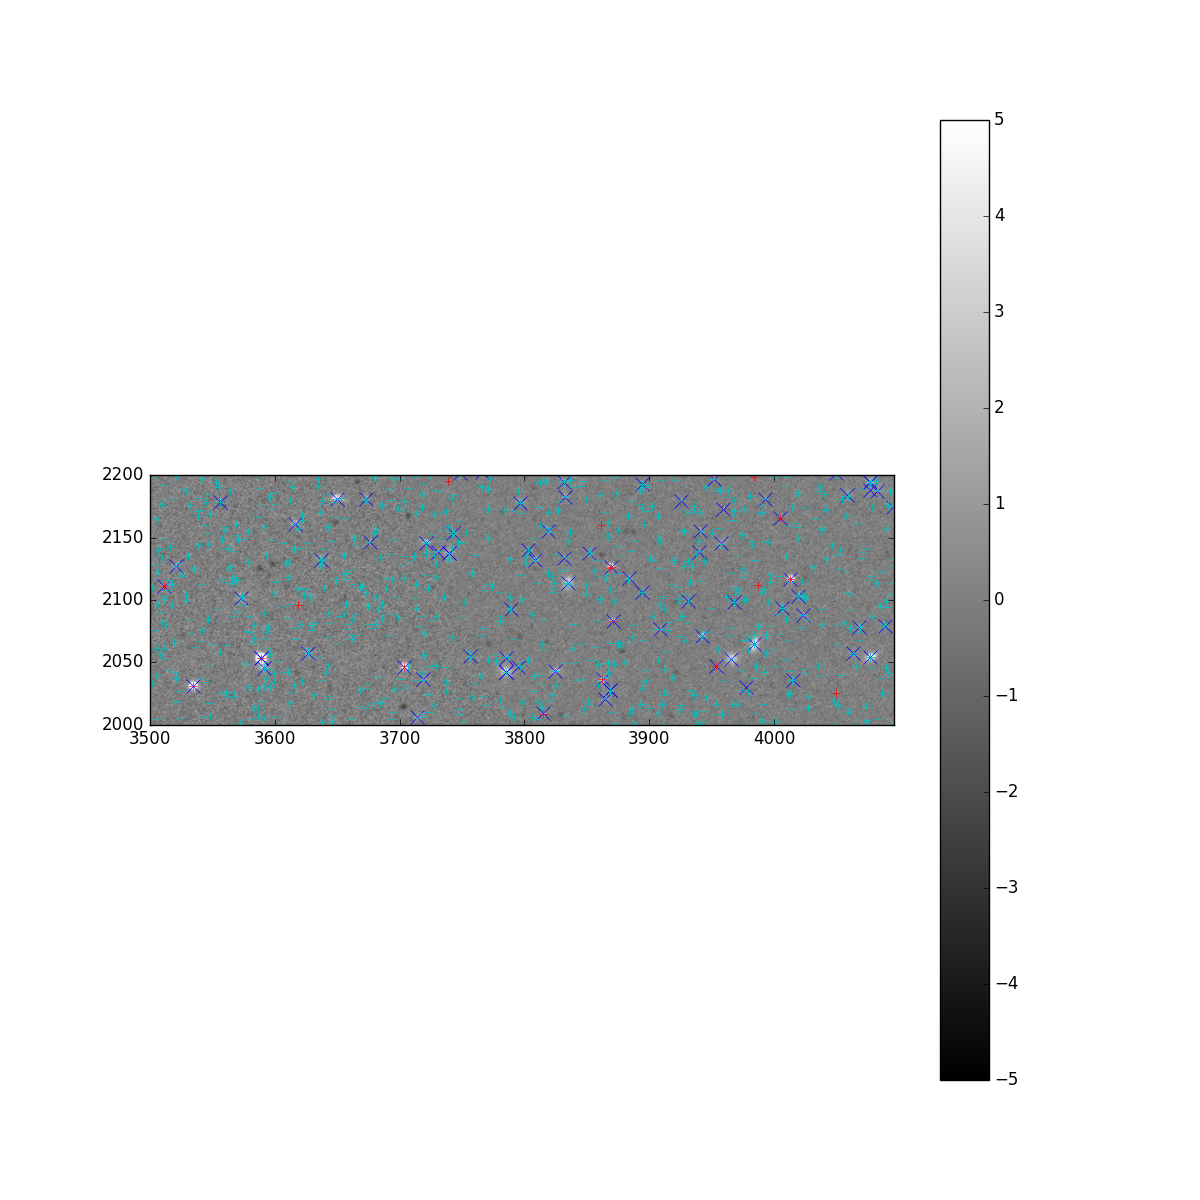
\includegraphics[width=0.9\columnwidth]{field.png}
\caption{Example of a 550 $\times$ 200 pixel simulated field. The axes show the pixel number in the CCD. The input galaxies are marked with cyan $+$, the input stars are marked with red $+$, and the detected sources are marked with blue $\times$. We can appreciate the vast difference in density between the simulation and the output given that CatSim contains objects fainter than what LSST can detect.}
\label{fig:coadd_example}
\end{figure}

\section{Quality checks}
\label{sec:quality}

One of the goals of this exercise is to check the quality and status of all pieces in the catalog generation and analysis process, and afterwards, check the capabilities and quality of the science working groups analysis pipelines. The first step is to match the input and output catalogs. In order to do that we generate a three-dimensional position and magnitude based tree using the \texttt{sklearn} package. Once the sources are matched we perform basic tests such as checking the differences between positions, redshift, and magnitudes, and their distributions. The results of these checks can be seen at \figref{basic_tests}. \CHECK{Generate more plots like this}.

\begin{figure}
\centering
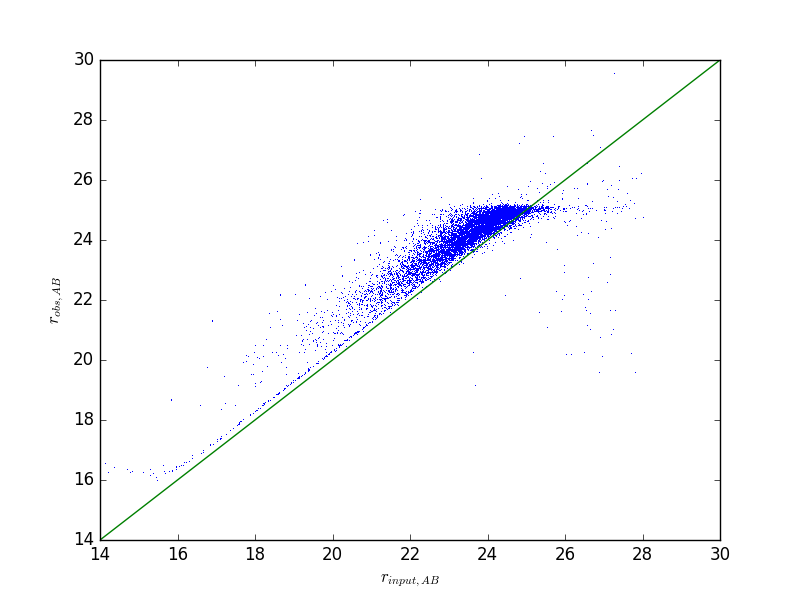
\includegraphics[width=0.9\columnwidth]{mag_scatter.png}
\caption{Scatter plot showing the observed r-band magnitude for the detected sources in the vertical axis and their input r-band magnitude.}
\label{fig:basic_tests}
\end{figure}

% ----------------------------------------------------------------------

\section{Masking procedure}
\label{sec:masking}

In this section we are going to present the methodology followed to prepare a mask to perform the clustering analysis.

\subsection{Bright objects masking}

Bright objects produce significant effects in the image that affects the detection and measurement of neighboring objects. Some examples of the effect of these objects are: saturation of the CCD, large diffraction spikes, obscuration of neighboring sources, etc. Thus, masking a region around these sources makes a more complicated footprint but largely simplifies the analysis of systematic effects. In order to evaluate the effect of this sources, we use the stars from the input catalog, we divide them in different magnitude bins, and we count the detected objects in a given radius. \CHECK{It has been suggested to count the detected objects in a given direction for certain distance because there are direction-dependent effects.} However, the number of objects in a given radius is dependent of the number of stars in each bin and subject to statistical fluctuations. Therefore, we use instead the average on this number for the different magnitude bins. This analysis is largely simplified if we use the numerical derivative of this quantity. In \figref{galdens_derivative} we can see that there is an excess of sources at distances lower than 10 arcseconds for the brightest stars. This is mainly due to the existence of fake sources around these bright objects. The brighter sources also have a larger noise, the DM deblender models the brightest source and subtracts this model looking for fainter sources that can be blended together with it. However, sometimes there are large noise peaks that have not been subtracted. These large noise peaks are detected in later stages as individual sources giving as a result these fake sources. \CHECK{Perform similar tests and establish a threshold (or thresholds) of distance to bright objects. Show a plot with fake sources.}.

\begin{figure}
\centering
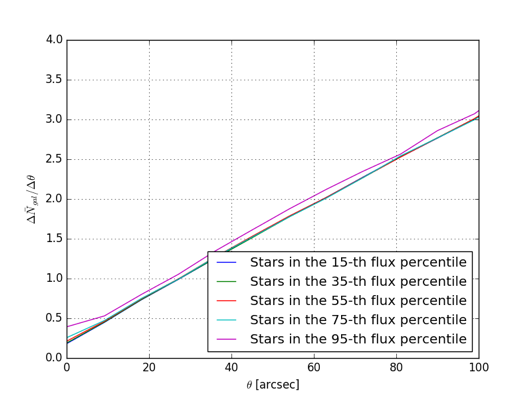
\includegraphics[width=0.9\columnwidth]{dngal_dtheta.png}
\caption{Mean increment in the number of detected objects around stars in the 95th flux percentile (magenta), the 75th percentile (cyan), the 55th percentile (red), the 35th percentile (green) and the 15th percentile (blue).}
\label{fig:galdens_derivative}
\end{figure}

% ----------------------------------------------------------------------

\section{Clustering results}
\label{sec:results}

Once we produce the mask we can proceed to measure the clustering statistics for our samples. One way to maximize this information is by characterizing the potential instrumental and systematic effects by using a transfer function. The fact that we have these realistic simulations allows us to compare the input \textit{truth} catalog to the output catalog which has been affected by these effects. We will analyze the transfer function using two different tools: the two point correlation function, and the angular power-spectrum. \CHECK{Describe the procedures and codes to measure these quantities, i.e, Landy-Szalay, ML-estimator, etc.}


\begin{figure}
\centering
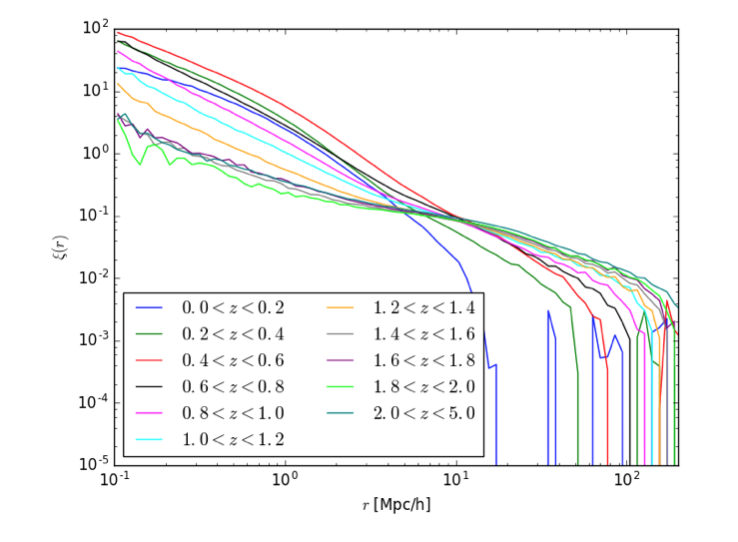
\includegraphics[width=0.9\columnwidth]{input_cf.png}
\caption{Input two point correlation function for different redshift bins. We assume a Planck $\Lambda$CDM model to compute the comoving distances.}
\label{fig:input_corr}
\end{figure}

\subsection{Systematic effects}

In this section we analyze the different systematic effects affecting the DC1 data.



% ----------------------------------------------------------------------

\section{Conclusions}
\label{sec:conclusions}

In this paper we presented the methodology to characterize the transfer function of LSST. This methodology can be easily exported to different photometric surveys. First, we performed a quality assessment of the data produced by the pipeline. Then, we generated the mask to perform our clustering analyses. Finally we compared the input and output two point clustering statistics to characterize the transfer function. \CHECK{Add more things when we have more results}.


% ----------------------------------------------------------------------

\subsection*{Acknowledgments}

Here is where you should add your specific acknowledgments, remembering that some standard thanks will be added via the \code{acknowledgments.tex} file.

%
The DESC acknowledges ongoing support from the Institut National de Physique Nucl\'eaire et de Physique des Particules in France; the Science \& Technology Facilities Council in the United Kingdom; and the Department of Energy, the National Science Foundation, and the LSST Corporation in the United States.  DESC uses resources of the IN2P3 Computing Center (CC-IN2P3--Lyon/Villeurbanne - France) funded by the Centre National de la Recherche Scientifique; the National Energy Research Scientific Computing Center, a DOE Office of Science User Facility supported by the Office of Science of the U.S.\ Department of Energy under Contract No.\ DE-AC02-05CH11231; STFC DiRAC HPC Facilities, funded by UK BIS National E-infrastructure capital grants; and the UK particle physics grid, supported by the GridPP Collaboration.  This work was performed in part under DOE Contract DE-AC02-76SF00515.
This manuscript has been authored by Fermi Research Alliance, LLC under Contract No. DE-AC02-07CH11359 with the U.S. Department of Energy, Office of Science, Office of High Energy Physics.

% 


%{\it Facilities:} \facility{LSST}

% Include both collaboration papers and external citations:
\bibliography{lsstdesc,main}

\end{document}
% ======================================================================
%
